\section{Zasady działania kompasu. Zofia Sosińska}\label{chap:naw}

Projekt kompasu jest na tyle prosty, aby nie przytłoczyć gracza nadmierną liczbą bodźców. Składa się horyzontalnego, jednolitego paska, na którym wyświetlane będą najważniejsze informacje o otoczeniu, symbol ośmiokąta, wskazujący na przestrzeń znajdującą się centralnie przed bohaterem, oraz z bocznych pasków, wyróżniających końce narzędzia.

\begin{figure}[htbp]
    \centering
    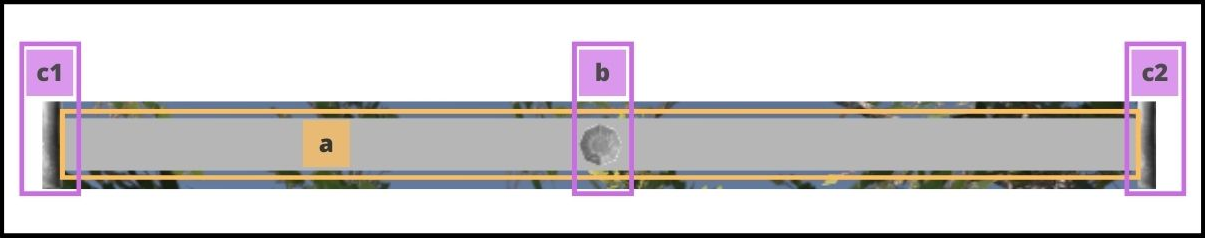
\includegraphics[width=0.9\textwidth]{images/ui/opis_ekementow_kompasu.png}
    \caption{Rozpiska elementów: a. główny pasek, b. symbol środka, c1., c2. paski końców kompasu.}\label{fig:compass_design}
\end{figure}

Ikony wyświetlane na kompasie będą przedstawiać najważniejsze informacje w polu widzenia gracza, czyli stronę świata, w kierunku której jest on zwrócony, oraz przeciwników.
Poniżej przedstawiono kod odpowiedzialny za wyznaczenie pozycji symbolu na omawianym narzędziu. Wejściem jest komponent RectTransform symbolu przypisanemu danemu obiektowi oraz jego położenie. Po obliczeniu wektora prowadzącego do uzyskania np. pozycji wroga, wyznaczany jest kąt, o jaki musi się obrócić. To przelicamy na pozycję na kompasie i, jeśli obiekt jest w polu widzenia, wyświatlamy symbol.

\begin{lstlisting}[caption=Fragment kodu odpowiedzialny za ustawienie symbolu na pasku kompasu]
void SetMarkerPosition(RectTransform markerTransform, Vector3 worldPosition)
{
    Vector3 dirToTarget = worldPosition - CameraTransform.position;
    float angle = Vector2.SignedAngle(
        new Vector2(dirToTarget.x, dirToTarget.z), 
        new Vector2(CameraTransform.transform.forward.x, 
        CameraTransform.transform.forward.z));
    float compassPositionX = Mathf.Clamp(
        2 * angle / Camera.main.fieldOfView, -1, 1);
    if (compassPositionX == 1 || compassPositionX == (-1))
    {
        markerTransform.anchoredPosition = new Vector2(0, 100);
    }
    else
    {
        markerTransform.anchoredPosition = new Vector2(
            compassBarTransform.rect.width / 2 * compassPositionX, 0);
    }
}
\end{lstlisting}

Problem lokalizacji stron świata pojawił się, gdy nieprawidłowe położenie na kompasie nieprawidłowo wyświetlały się symbole po użyciu najprostszego rozwiązania. Było to pobranie wartości od Vector3.forward, co jest skrótowym zapisem Vector3(0, 0, 1). Lewy dolny róg mapy jest położony w punkcie (0, 0, 0), co oznacza, że wymagane jest przesunięcie, aby prawidłowo zasymulować strony świata. Płnoc i Południe przesunęliśmy do połowy szerokości, a Wschód i Zachód - długości mapy. Każde z nich odaliliśmy o 60000 jednostek, co pozwala na wiarygodą symulację stron świata na kompasie.
\begin{figure}[htbp]
    \centering
    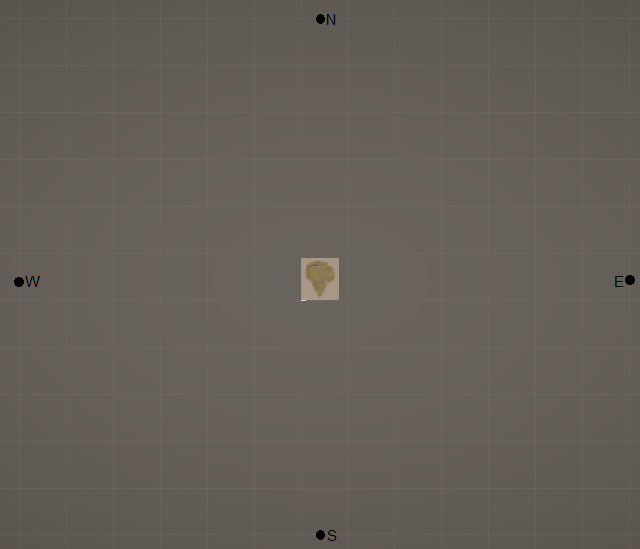
\includegraphics[width=0.9\textwidth]{images/ui/strony_swiata.png}
    \caption{Rozmieszczenie zasymulowanych stron świata.}\label{fig:world_sides}
\end{figure}

Wykrycie wrogich jednostek znajduje się w funkcji Start. Każdemu obiektowi jest przypisywany symbol czerwonego miecza i w zależności od położenia wroga, obrazek wyświetlany jest odpowiednio na kompasie.
\begin{lstlisting}[caption=Fragment kodu odpowiedzialny za połączenie wrogich obiektów na mapie z symbolami wyświetlonymi na kompasie]
    void SetPositionOfEnemies()
    {
        foreach (
            var e in enemiesOnMap.Zip(
                enemiesOnUI, (x, y) => new { 
                    enemyOnMap = x, enemyOnUI = y }))
        {
            SetMarkerPosition(
                e.enemyOnUI.GetComponent<RectTransform>(),
                e.enemyOnMap.transform.position);
        }
    }
\end{lstlisting}